\section{Qualitätssystem}

\begin{tcolorbox}[title=Qualitätssystem]
    Aufgrund der typischen schrittweisen Konkretisierung von Qualitätsforderungen sind Qualitätssysteme  \textit{hierarchisch} aufgebaut:

    \begin{itemize}
        \item \textbf{Qualität} wird definiert durch
        \begin{itemize}
            \item  \textbf{Qualitätsmerkmale} (bspw. ``\textit{Effizienz}``), die konkretisiert werden durch
            \begin{itemize}
                \item  \textbf{Qualitätsteilmerkmale} (bspw. ``\textit{Performance}``, ``\textit{Verbrauchsverhalten}``), die genau definiert werden durch
                \begin{itemize}
                    \item \textbf{Qualitätsindikatoren}, die jeweils einem \textit{Artefakt} innewohnende Eigenschaften beschreibt, die objektiv bestimmt werden kann (bspw. ``\textit{Antwortzeit}``, ``\textit{Datendurchsatz}``)
                \end{itemize}
            \end{itemize}
        \end{itemize}
    \end{itemize}

    \noindent
    Zur Bestimmung von Qualitätsindikatoren werden \texbf{Metriken} eingesetzt, also ``\textit{Vorschriften}, anhand derer Zahlen berechnet werden können, die ein Maß für die Güte einer Software darstellen`` (\cite[3, Hervorhebung eigene]{Wed09c}).
\end{tcolorbox}


\begin{figure}
    \centering
    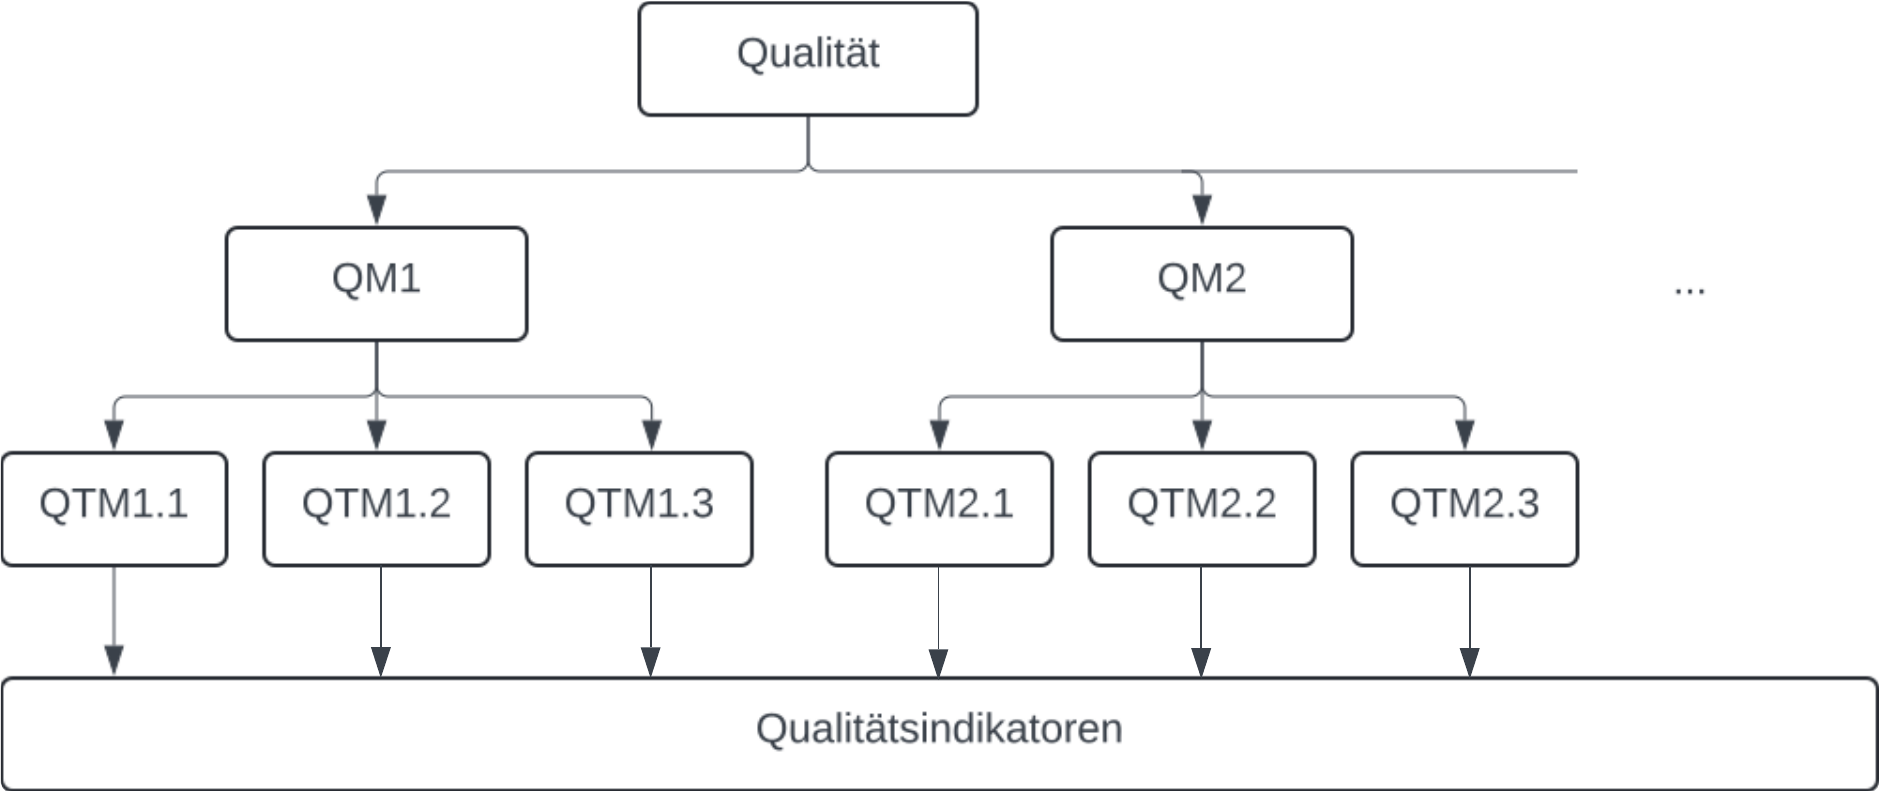
\includegraphics[scale=0.8]{part four/Qualität/img/qualitätssysteme}
    \caption{Skizzenhafter Aufbau von Qualitätssystemen. \textit{Qualitätsindikatoren} sind als breiter Balken dargestellt, da sich mehrere \textit{Qualitätsteilmerkmale} auf einen gemeinsamen \textit{Qualitätsindikator} beziehen können. (Quelle: in Anlehnung an~\cite[Abb. 1.1, 3]{Wed09c})}
    \label{fig:qualitätssysteme-cc}
\end{figure}